
\chapter{Simulations}\label{chapter:simulations}

In this chapter I want to give an intuition for the results on no-regret convergence in finite games discussed in chapter \ref{chapter:literatureReview}. I have implemented both, \textit{projected online gradients ascent} (POGA) and \textit{entropic gradient ascent} (EGA). As expected both algorithms show very similar behavior. The \textit{steep entropic regularizer} used in EGA slightly reshaped space in comparison to the common \textit{Euclidean regularizer} in POGA. In terms of convergence, however, both behave identically. For that reason, I might show plots of only one algorithm. In the vector flied plots the black star ($\bigstar$) will denote a an interior Nash equilibrium while the black dot ({\Large\textbullet}) stands for a pure Nash equilibrium. The orange dot ({\color[HTML]{E37222}\Large\textbullet}) denotes an initial strategy profile. \\

As the results suggested I found Nash convergence in frequencies in two player zero sum games with interor equilibria and last-iterate convergence in games were strict Nash equilibria exist. I have limited myself on 2x2 and 3x3 bimatrix games as higher dimensional games with more than two players are hard to illustrate. Therefore we have $\mathcal{N} = \{1,2\}$ throughout this chapter. The outcome of no-regret learning depends on the type of game and the type of equilibria. The chapter is structured accordingly. 

\section{Unique Fully Mixed Nash Equilibrium}\label{section:uniqueMixedNashEquilibrium}

Let us first consider games that yield an interior, or equivalently fully mixed, Nash equilibrium. In general we would expect the algorithms' trajectories not to converge because there exists no pure and therefore no strict Nash equilibrium. However in two player zero sum games at least we expect the empirical frequency of play, i.e. time averaged strategies, to converge to the interior Nash equilibrium (proposition \ref{prop:empiricalFrequencyConvergence}).

\subsection{Matching Pennies}\label{subsection:machtingPennies}

Matching Pennies is a simple two player zero sum game. Both player choose between \textit{Heads} and \textit{Tails} and if they match then the row player wins and if they mismatch the column player wins. The payoff is set accordingly as in \ref{tab:payoffMachtingPennies}. 

\begin{table}[H]\centering
\setlength{\extrarowheight}{2pt}
\begin{tabular}{cc|c|c|}
  & \multicolumn{1}{c}{} & \multicolumn{1}{c}{$Heads$}  & \multicolumn{1}{c}{$Tails$} \\\cline{3-4}
  & $Heads$ & $1,-1$ & $-1,1$ \\\cline{3-4}
  & $Tails$ & $-1,1$ & $1,-1$ \\\cline{3-4}
\end{tabular}\caption{\label{tab:payoffMachtingPennies}payoff matrix Matching Pennies}
\end{table}

There is only a single fully mixed Nash equilibrium, i.e. when both players chooses \textit{Heads} and \textit{Tails} equally likely. 

\begin{equation*}
    x_{i}^{*} = (1/2,1/2) \qquad \forall i \in \mathcal{N}
\end{equation*}

As stated in proposition \ref{prop:noInteriorStable} no fully mixed strategy, and therefore no interior Nash equilibrium, can be stable under \ref{equ:FTRL} algorithms. Since \ref{equ:FTRL} can only converge to stable states or strict Nash Equilibira equivalently (see proposition \ref{prop:StrictStableEquivalent}), for both EGA and POGA the induced sequence of play fail to converge. In fact both exhibit finite cyclic behaviour around the unique MNE as illustrated in the figure \ref{fig:PenniesStream1}. As we can see, using entropic regularization the projections always lead to interior strategies whereas for Euclidean regularization we obtain potential Euclidean projections to the boundary. Note that $x_{i,Tails}$ is implicitly given by $1 - x_{i,Heads}$.

\begin{figure}[H]
\centering
\begin{subfigure}{.5\textwidth}
    \centering
    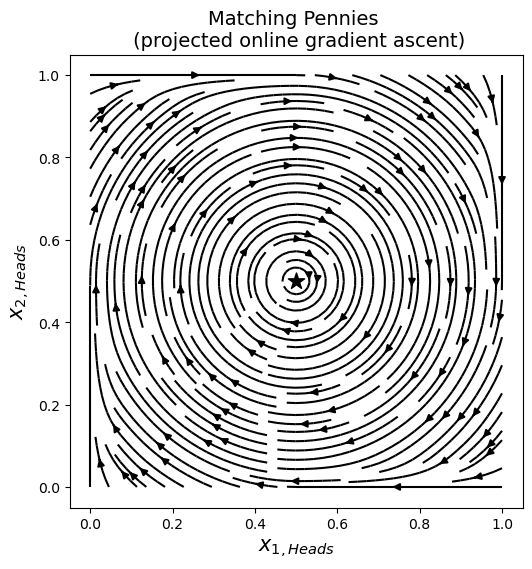
\includegraphics[width=\textwidth]{logos/Pennies1.png}
    \caption{POGA}
\end{subfigure}%
\begin{subfigure}{.5\textwidth}
    \centering
    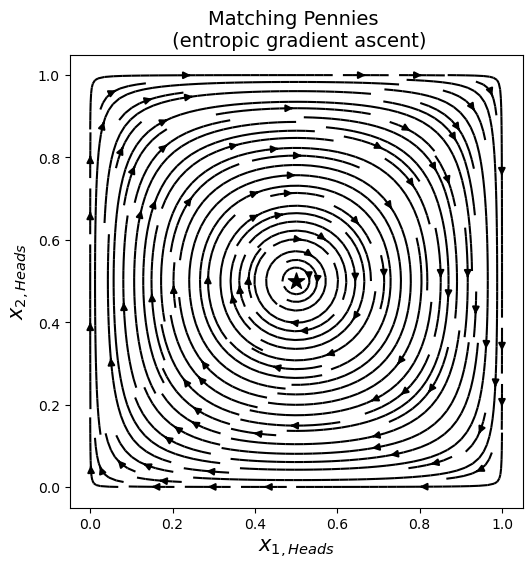
\includegraphics[width=\textwidth]{logos/Pennies2.png}
    \caption{EGA}
\end{subfigure}
\caption{vector field in Matching Pennies}
\label{fig:PenniesStream1}
\end{figure}

A closer examination of the specific trajectories induced by the algorithms we find that actually they are repelled from the interior equilibrium as depicted in figure \ref{fig:PenniesDivergence}. As mentioned earlier in every 2x2 zero sum game with interior equilibrium, trajectories diverge to the boundary under \ref{equ:FTRL} for all initial strategy profiles other than the equilibrium \cite{bailey}. 


\begin{figure}[H]
 \captionsetup{justification=centering}
\centering
\begin{subfigure}{.5\textwidth}
    \centering
    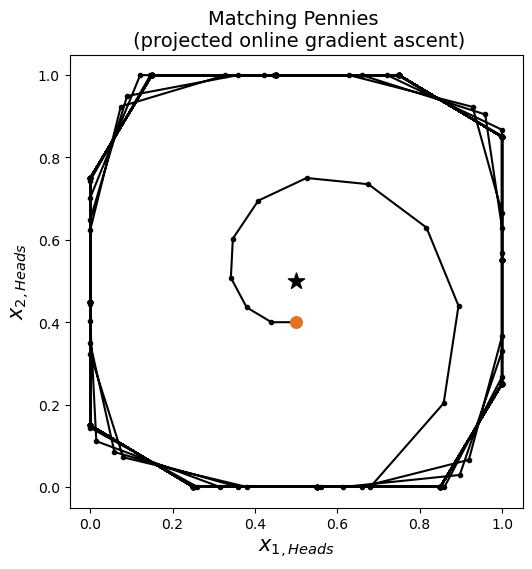
\includegraphics[width=\textwidth]{logos/Pennies5.png}
    \caption{POGA}
\end{subfigure}%
\begin{subfigure}{.5\textwidth}
    \centering
    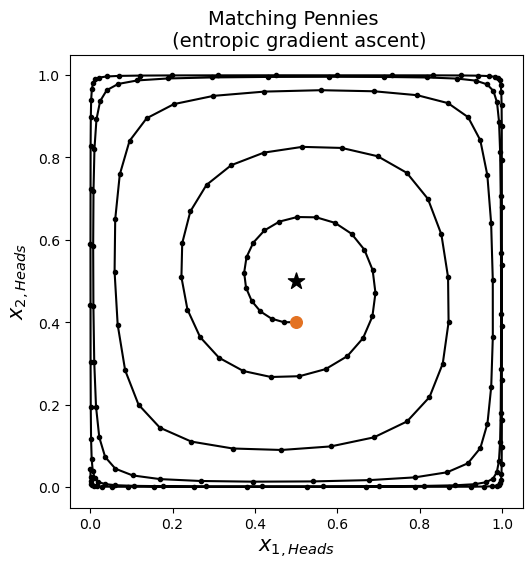
\includegraphics[width=\textwidth]{logos/Pennies6.png}
    \caption{EGA}
\end{subfigure}
\caption{trajectories with initial strategies $x_{1}^0 = (\frac{1}{2},\frac{1}{2})$ and $x_{2}^0 = (\frac{2}{5},\frac{3}{5})$, $T = 200$, $\gamma = 0.3$}
\label{fig:PenniesDivergence}
\end{figure}


The time averaged trajectories however, ultimately converge to the unique MNE. That happened independently from the initial strategies of the players. The amplitude of of cycles dampens over time as in figure \ref{fig:Pennies7}. That finding perfectly fits to proposition \ref{prop:empiricalFrequencyConvergence}.

\begin{figure}[H]
    \centering
    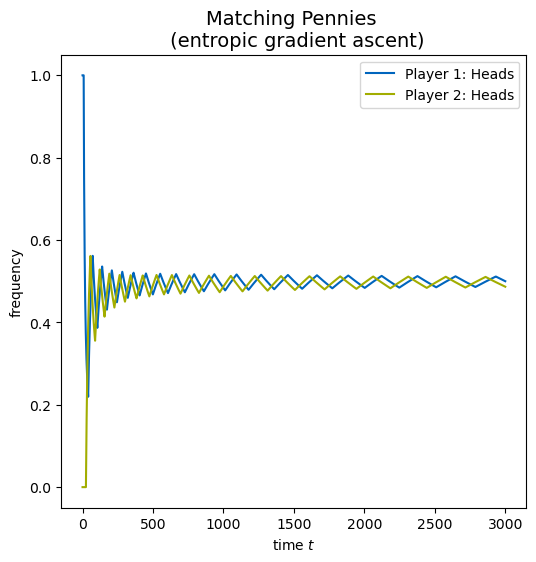
\includegraphics[width=0.5\textwidth]{logos/Pennies7.png}
    \caption{EGA empirical frequency of play in Matching Pennies, $\gamma = 0.1$}
    \label{fig:Pennies7}
\end{figure}


\subsection{Rock Paper Scissors}\label{subsection:rockPaperScissors}

One might think the convergence of empirical frequencies to the game's MNE is an artifact of its simple 2x2 structure, but I found similar behavior in Rock Paper Scissors, another zero-sum game.

\begin{table}[H]\centering
\setlength{\extrarowheight}{2pt}
\begin{tabular}{cc|c|c|c|}
  & \multicolumn{1}{c}{} & \multicolumn{1}{c}{$Rock$}  & \multicolumn{1}{c}{$Paper$}  & \multicolumn{1}{c}{$Scissors$} \\\cline{3-5}
            & $Rock$ & $0,0$ & $-1,1$ & $1,-1$ \\ \cline{3-5}
            & $Paper$ & $1,-1$ & $0,0$ & $-1,1$ \\\cline{3-5}
            & $Scissors$ & $-1,1$ & $1,-1$ & $0,0$ \\\cline{3-5}
\end{tabular}\caption{\label{tab:payoffRPS}payoff matrix Rock Paper Scissors}
\end{table}

The only Nash equilibrium that exists is the following fully mixed NE

\begin{equation*}
    x_{i}^{*} = (1/3,1/3,1/3) \qquad \forall i \in \mathcal{N}
\end{equation*}

Both algorithms exhibit finite out-of-sync oscillating behavior. Also the cyclic period and the amplitude increases over time which corresponds to the repelling behavior from figure \ref{fig:PenniesDivergence}. The players essentially chase one another. Again, the empirical frequencies, on the other hand, converge to the game's interior Nash equilibrium as in figure \ref{fig:RPS}. Note that the initial strategies are set randomly.

\begin{figure}[H]
\centering
\begin{subfigure}{.5\textwidth}
    \centering
    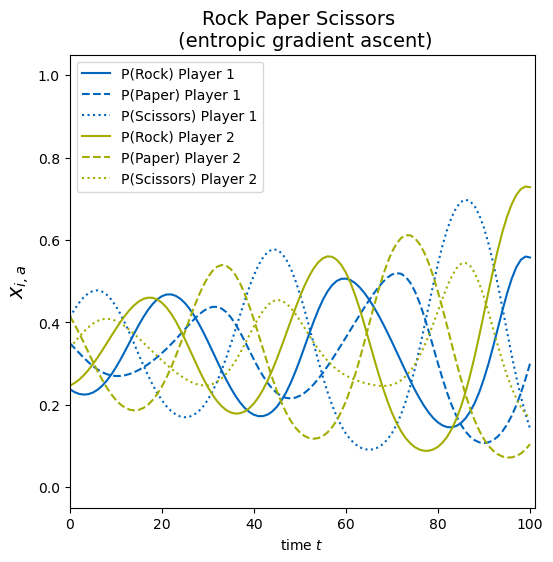
\includegraphics[width=\textwidth]{logos/RPS2.png}
    \caption{last iterate}
    %\label{fig:POGDpseudocode}
\end{subfigure}%
\begin{subfigure}{.5\textwidth}
    \centering
    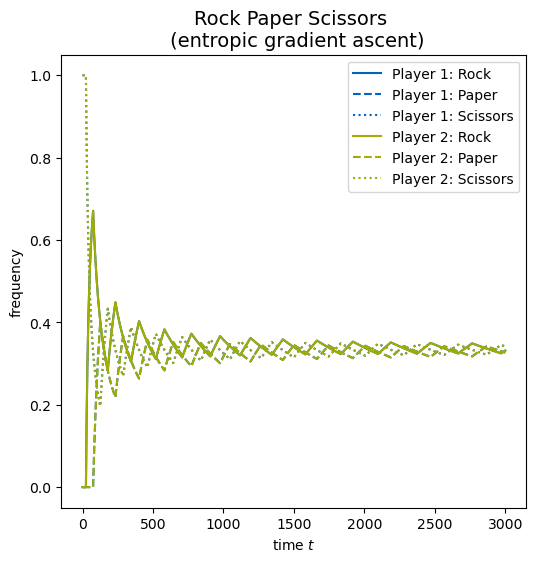
\includegraphics[width=\textwidth]{logos/RPS3.png}
    \caption{on average}
    %\label{fig:POGDpseudocode}
\end{subfigure}
\caption{EGA behavior in Rock Paper Scissors, $\gamma = 0.1$}
\label{fig:RPS}
\end{figure}


\subsection{Shapley Game}\label{subsection:shapleyGame}

The Shapley Game resembles that of Rock Paper Scissors. The difference is that it is not zero sum but general sum. In the payoff matrix in \ref{tab:payoffShapley} we can see that the utility of an action profile sometimes sums up to $1$ and sometimes to $0$. 

\begin{table}[H]\centering
\setlength{\extrarowheight}{2pt}
\begin{tabular}{cc|c|c|c|}
  & \multicolumn{1}{c}{} & \multicolumn{1}{c}{$L$}  & \multicolumn{1}{c}{$C$}  & \multicolumn{1}{c}{$R$} \\\cline{3-5}
            & $T$ & $1,0$ & $0,1$ & $0,0$ \\ \cline{3-5}
            & $M$ & $0,0$ & $1,0$ & $0,1$ \\\cline{3-5}
            & $B$ & $0,1$ & $0,0$ & $1,0$ \\\cline{3-5}
\end{tabular}\caption{\label{tab:payoffShapley}payoff matrix Shapley Game}
\end{table}

The game's unique NE is the same fully mixed Nash equilibrium as in Rock Paper Scissors

\begin{equation*}
    x_{i}^{*} = (1/3,1/3,1/3) \qquad \forall i \in \mathcal{N}
\end{equation*}

In this case, both EGA and POGA, are non convergent neither in weights nor in frequencies (figure \ref{fig:Shapley}). Again the weights cycle exponentially through the space of possible strategies. As far as frequencies are concerned the amplitudes of the cycles do not dampen over time as they did in Matching Pennies or Rock Paper Scissors. They rather grow exponentially. In general sum games, like the Shapley Game, no regret dynamics  seem to fail to converge generally. The same behaviour was found for \textit{fictitious play}, a simple \textit{best response} dynamic that is not a no regret algorithm \cite{jafari}.


\begin{figure}[H]
\centering
\begin{subfigure}{.5\textwidth}
    \centering
    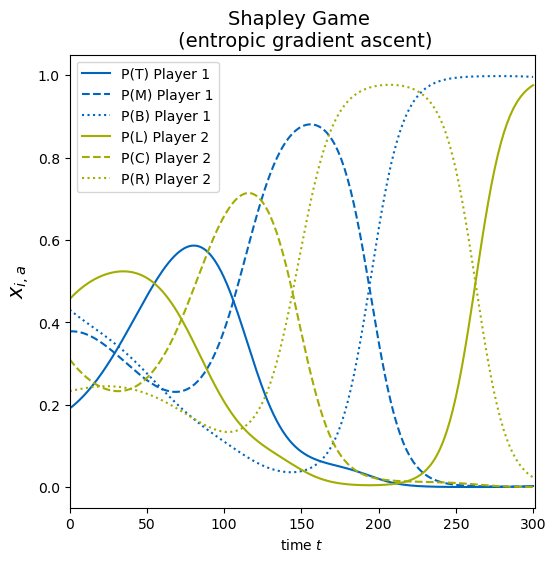
\includegraphics[width=\textwidth]{logos/Shapley1.png}
    \caption{last iterate}
    %\label{fig:POGDpseudocode}
\end{subfigure}%
\begin{subfigure}{.5\textwidth}
    \centering
    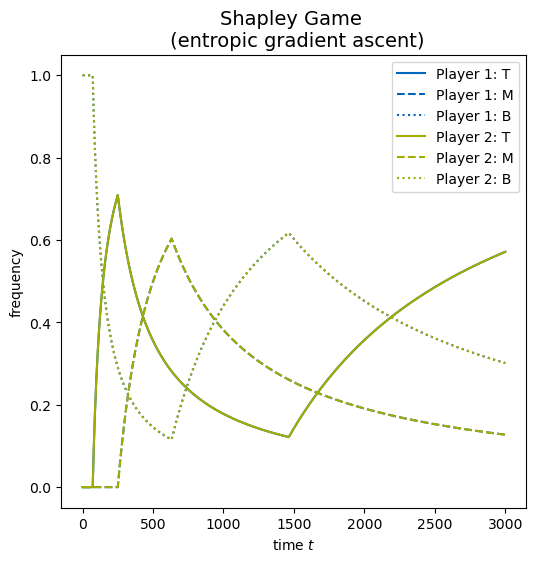
\includegraphics[width=\textwidth]{logos/Shapley2.png}
    \caption{on average}
    %\label{fig:POGDpseudocode}
\end{subfigure}
\caption{divergent behavior of EGA in Shapley Game, $\gamma = 0.1$}
\label{fig:Shapley}
\end{figure}


\section{Unique Pure Nash Equilibrium}\label{section:uniquePureNashEquilibrium}

Next, we consider games with an unique pure Nash equilibrium. One can easily verify that there is no game with an unique weak PNE and therefore the PNE must be strict in a sense of definition \ref{def:strictNE}. Therefore, we anticipate the unique PNE to be globally stable as defined in \ref{def:stability}. Hence, according to proposition \ref{prop:globalConvergence} we can expect that both algorithms' trajectories converge globally to the equilibrium.  

\subsection{Prisoner's Dilemma}\label{subsection:prisonersDilemma}

The example I would like to address is the famous Prisoner's Dilemma. The game works as follows. Two bank robbers have been arrested. They are separated from each other and both can choose either to stay silent or to betray the other one by admitting the crime. When both stay silent, both are sent to prison for only one year. When both betray they go to jail for 2 years each. However, if one stays silent while the other betrays the one that stayed silent goes is sent to prison for 3 years while the other one is set free, see table \ref{tab:payoffPrisoners}.

\begin{table}[H]\centering
\setlength{\extrarowheight}{2pt}
\begin{tabular}{cc|c|c|}
  & \multicolumn{1}{c}{} & \multicolumn{1}{c}{$Silent$}  & \multicolumn{1}{c}{$Betray$} \\\cline{3-4}
  & $Silent$ & $-1,-1$ & $-3,0$ \\\cline{3-4}
  & $Betray$ & $0,-3$ & $-2,-2$ \\\cline{3-4}
\end{tabular}\caption{\label{tab:payoffPrisoners}payoff matrix Prisoner's Dilemma}
\end{table}

The only Nash equilibrium is when both players always choose \textit{Betray}. So there is no fully mixed Nash equilibrium but only one pure Nash equilibrium. 

\begin{equation*}
    x^{*} = (Betray,Betray) \qquad \textit{strict }\text{PNE}
\end{equation*}

Note that the PNE is also strict. Any unilateral deviation from the PNE would lead to a reduction in payoff. For instance, if the row player knows that the column player  chooses \textit{Betray} then deviating from \textit{Betray} would decrease the \textit{row player's} payoff, from $-2$ to $-3$. As the game is symmetric the same holds for the column player. \\

Another observation is that for both players \textit{Silent} is dominated by \textit{Betray}. More precisely, no matter what the column players chooses to play, the row player is always better of playing \textit{Betray}, because $0 > -1$ and $-2 > -3$. Again, since the game is symmetric the same holds for the column player. So by iteratively eliminating dominated strategies we can solve this games. Such games are also called \textit{dominance solvable}. As stated in proposition \ref{prop:dominantedStrategiesExtinct} we expect that for both algorithms the dominated strategy \textit{Silent} becomes extinct, that means $x_{i,Silent}$ tends to $0$ as the number of iterations grows.  \\

Consider figure \ref{fig:Prisoner}. The blue region indicates strategies in the neighbourhood with respect to the PNE that fulfill the inequality from the definition of stable states (\ref{def:stability}). We can see the PNE is globally stable. As stated in proposition \ref{prop:globalConvergence} no-regret dynamics converge globally to the globally stable equilibrium. As the vector field suggests, both POGA and EGA indeed converges globally to the games's unique PNE. Also the dominated strategy \textit{Silent} becomes extinct.


\begin{figure}[H]
\captionsetup{justification=centering}
\centering
\begin{subfigure}{.5\textwidth}
    \centering
    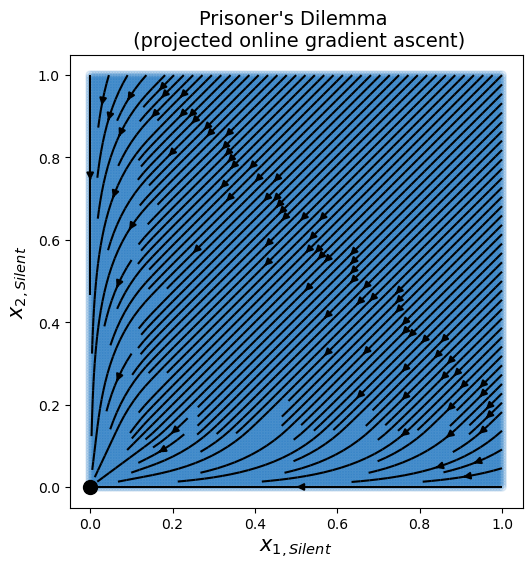
\includegraphics[width=\textwidth]{logos/Prisoner2.png}
    \caption{EGA}
    %\label{fig:POGDpseudocode}
\end{subfigure}%
\begin{subfigure}{.5\textwidth}
    \centering
    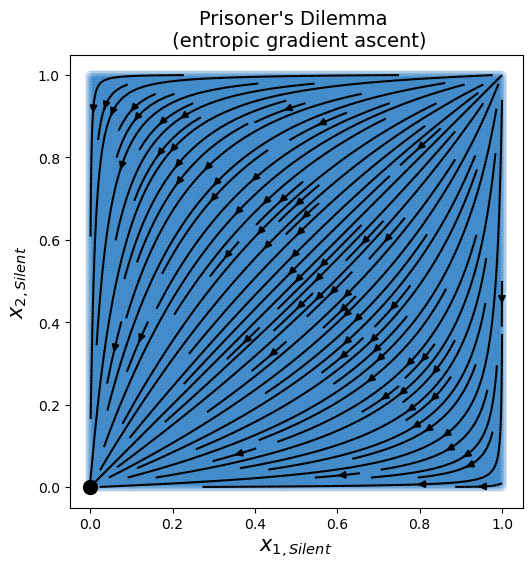
\includegraphics[width=\textwidth]{logos/Prisoner3.png}
    \caption{POGA}
    %\label{fig:POGDpseudocode}
\end{subfigure}
\caption{vector field in Prisoner's Dilemma the blue region indicates the stable neighbourhood w.r.t the PNE}
\label{fig:Prisoner}
\end{figure}

Considering some specific trajectories that the algorithms take shown in figure \ref{fig:Prisoner2}, we find that in EGA does not reach the boundary as the projections always lead to interior strategies using entropic regularization. For OPGA, on the other hand, the Euclidean projections lead to strategies on the boundary at some point. Interestingly using the same step size of $\gamma = 0.1$ POGA descent converges much faster than EGA. 

\begin{figure}[H]
\captionsetup{justification=centering}
\centering
\begin{subfigure}{.5\textwidth}
    \centering
    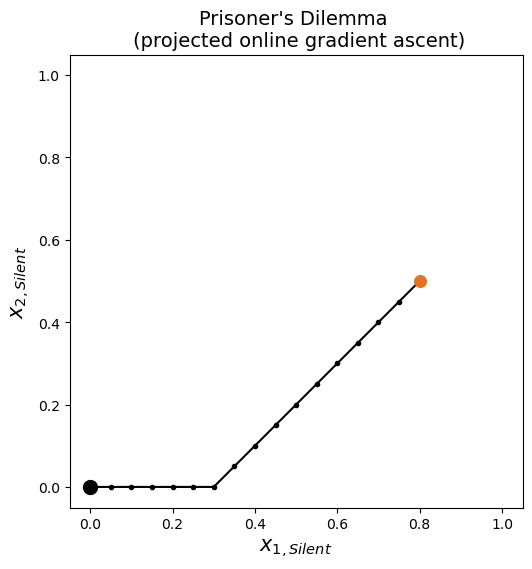
\includegraphics[width=\textwidth]{logos/Prisoner4.png}
    \caption{EGA}
    %\label{fig:POGDpseudocode}
\end{subfigure}%
\begin{subfigure}{.5\textwidth}
    \centering
    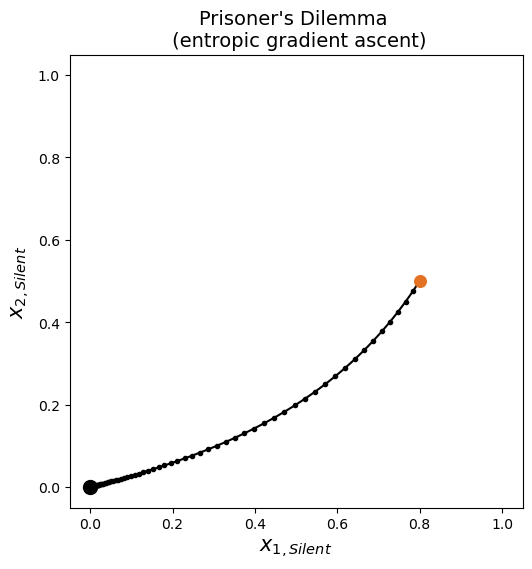
\includegraphics[width=\textwidth]{logos/Prisoner5.png}
    \caption{POGA}
    %\label{fig:POGDpseudocode}
\end{subfigure}
\caption{trajectories with initial strategies $x_{1}^0 = (\frac{4}{5},\frac{1}{5})$ and $x_{2}^0 = (\frac{1}{2},\frac{1}{2})$, $T = 200$, $\gamma = 0.3$}
\label{fig:Prisoner2}
\end{figure}


\section{Mixed and Pure Nash Equilibria}\label{section:MixedandPureNashEquilibria}

In games where both fully mixed and pure Nash equilibria exist, we expect no-regret algorithms to converge to strict pure Nash equilibria solely. We will see that as mentioned in proposition \ref{prop:noInteriorStable} that interior equilbria are not asymptotically stable and therefore not attracting.

\subsection{Battle Of Sexes}\label{subsection:battleOfSexes}

Image a couple of two persons with different interests. One would prefer to watch a boxing fight, say the row player, and the other one prefers to go to a ballet, the column player. But they would rather spend time together than choosing different events. There is no communication between both. The payoff is set accordingly as in table \ref{tab:payoffBattleOfSexes}.

\begin{table}[H]\centering
\setlength{\extrarowheight}{2pt}
\begin{tabular}{cc|c|c|}
  & \multicolumn{1}{c}{} & \multicolumn{1}{c}{$Fight$}  & \multicolumn{1}{c}{$Ballet$} \\\cline{3-4}
  & $Fight$ & $3,2$ & $0,0$ \\\cline{3-4}
  & $Ballet$ & $0,0$ & $2,3$ \\\cline{3-4}
\end{tabular}\caption{\label{tab:payoffBattleOfSexes}payoff matrix Battle of Sexes}
\end{table}

There are two quite obvious pure Nash equilibria. One where both choose \textit{Fight}, and one where both choose \textit{Ballet}. But there is also a fully mixed Nash equilibrium, i.e when both players randomize over the actions. In particular the row player should choose \textit{Fight} with probability $2/3$ and \textit{Ballet} with $1/3$ and the column player should choose \textit{Fight} with $1/3$ and \textit{Ballet} with $2/3$. In formulas we have the following Nash equilibria

\begin{description}\centering
    \item $x^{*} = (Fight,Fight) \qquad \textit{strict }\text{PNE}$
    \item $x^{*} = (Betray,Betray) \qquad \textit{strict }\text{PNE}$
    \item $x_{1}^* = (2/3,1/3) \qquad x_{2}^* = (1/3,2/3) \qquad \text{MNE}$
\end{description}

Note that again both PNEs are strict in a sense of definition \ref{def:strictNE}. Neither the row player nor the column player can unilaterally deviate from an PNE without reducing its payoff. According to proposition \ref{prop:StrictStableEquivalent} that means both PNE are also stable states as defined in \ref{def:stability}. Then both PNEs must also be locally attracting (proposition \ref{prop:localConvergence}). And indeed, as shown in figure \ref{fig:BOS1}, both algorithms converge locally to the corresponding PNE. Notice how the stable regions of the PNEs intersect.

\begin{figure}[H]
\captionsetup{justification=centering}
\centering
\begin{subfigure}{.5\textwidth}
    \centering
    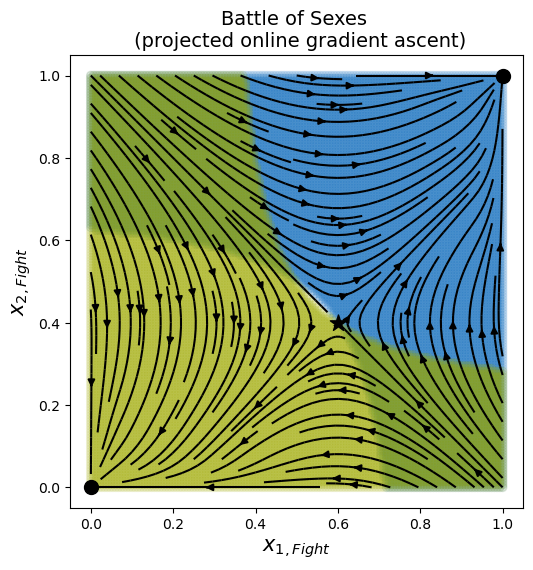
\includegraphics[width=\textwidth]{logos/BattleOfSexes1.png}
    \caption{EGA}
    %\label{fig:POGDpseudocode}
\end{subfigure}%
\begin{subfigure}{.5\textwidth}
    \centering
    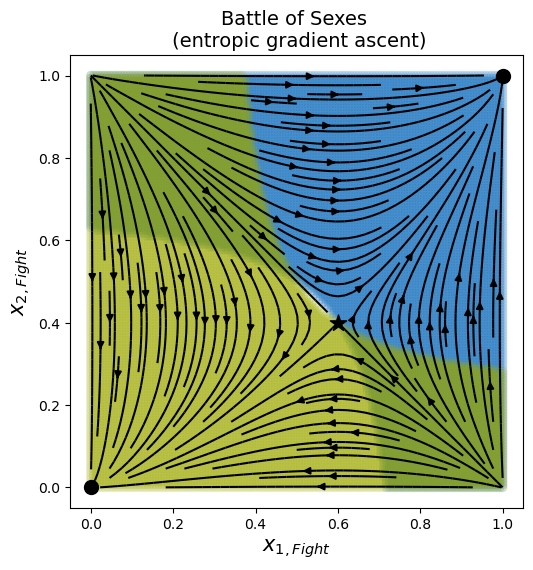
\includegraphics[width=\textwidth]{logos/BattleOfSexes2.png}
    \caption{POGA}
    %\label{fig:POGDpseudocode}
\end{subfigure}
\caption{vector field in Prisoner’s Dilemma using POGA (left) and EGA (right),
the blue region indicates the stable neighbourhood w.r.t \textit{(Fight,Fight)} and light green w.r.t to \textit{(Ballet,Ballet)}, the dark green region is the intersection of both}
\label{fig:BOS1}
\end{figure}

For clarification I have highlighted only the stable neighbourhood with respect to the PNE \textit{(Fight,Fight)} in figure \ref{fig:BOS2a}. Also notice that not all points in the stable region converge to the corresponding PNE. For an example refer to \ref{fig:BOS2b} In this game, for instance, all initial point above the diagonal between \textit{(Fight,Ballet)} and \textit{(Ballet,Fight)} converge to the PNE \textit{(Fight,Fight)} and all point below converge to the PNE \textit{(Ballet,Ballet)}.


\begin{figure}[H]
\captionsetup{justification=centering}
\centering
\begin{subfigure}{.5\textwidth}
    \centering
    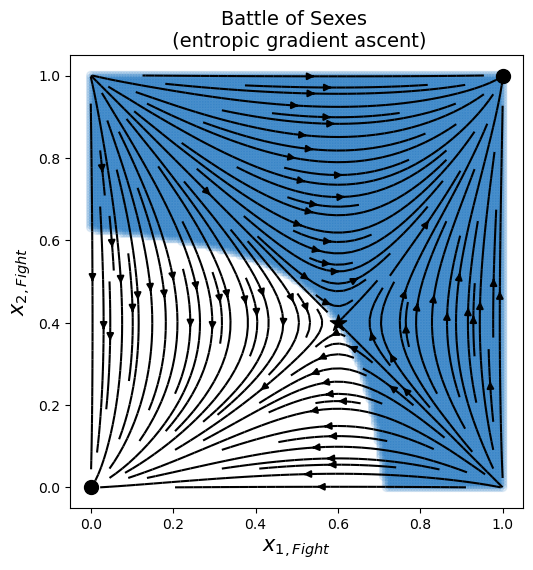
\includegraphics[width=\textwidth]{logos/BattleOfSexes3.png}
    \caption{stable neighbourhood w.r.t \textit{(Fight,Fight)}}
    \label{fig:BOS2a}
\end{subfigure}%
\begin{subfigure}{.5\textwidth}
    \centering
    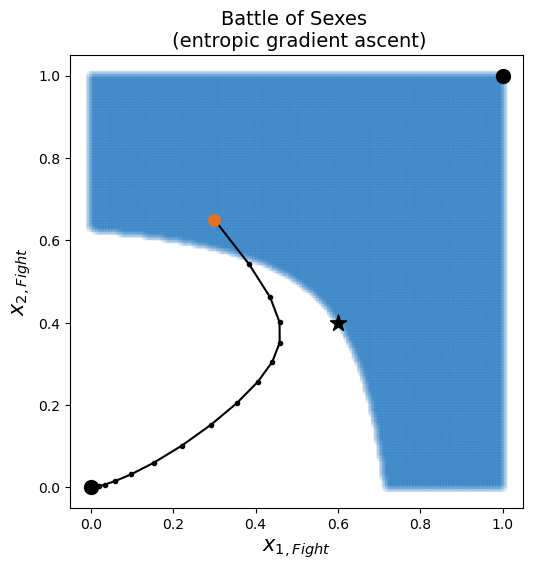
\includegraphics[width=\textwidth]{logos/BattleOfSexes4.png}
    \caption{$x_{1}^0 = (0.3,0.7)$, $x_{2}^0 = (0.65,0.35)$, $T = 200$}
    \label{fig:BOS2b}
\end{subfigure}
\caption{EGA in Battle of Sexes, $\gamma = 0.1$}
\label{fig:BOS2}
\end{figure}

The question might raise whether the fully mixed Nash equilibrium can be stable as well. Even though there is a stable region for the MNE as depicted in \ref{fig:BOS3a}, we cannot find a neighborhood for the MNE such that the inequality of the stability definition (\ref{def:stability}) holds for all strategies within the neighbourhood. Intuitively, no matter how far we zoom in to the MNE we cannot draw a circle around it such that all points within the circle are blue as illustrated in figure \ref{fig:BOS3b}. Therefore except from the perfect diagonal between \textit{(Fight,Ballet)} and \textit{(Ballet,Fight)} the algorithms never converges towards the interior Nash equilibrium. The same behavior was observed for POGA. That is align with proposition \ref{prop:noInteriorStable} that no interior point can be stable under \ref{equ:FTRL}. 

\begin{figure}[H]
\captionsetup{justification=centering}
\centering
\begin{subfigure}{.5\textwidth}
    \centering
    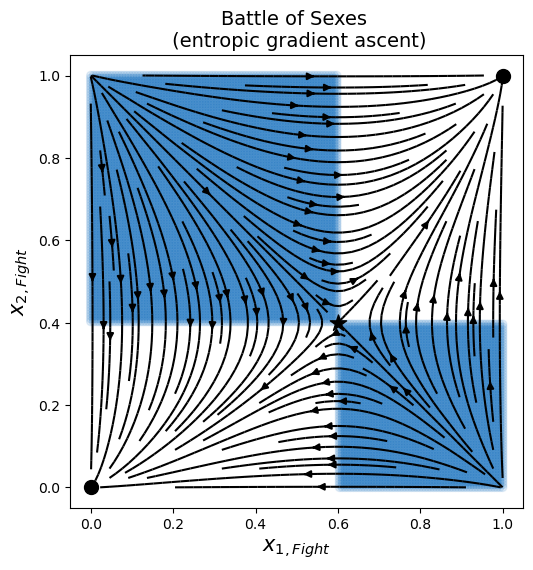
\includegraphics[width=\textwidth]{logos/BattleOfSexes6.png}
    \caption{stable neighbourhood w.r.t equilibrium}
    \label{fig:BOS3a}
\end{subfigure}%
\begin{subfigure}{.5\textwidth}
    \centering
    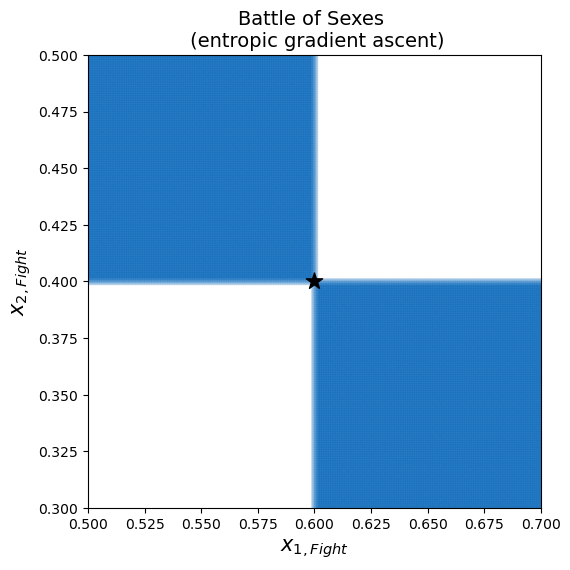
\includegraphics[width=\textwidth]{logos/BattleOfSexes5.png}
    \caption{zoomed in to the interior equilibrium}
    \label{fig:BOS3b}
\end{subfigure}
\caption{The interior equilibrium is not stable under EGA in Battle of Sexes}
\label{fig:BOS3}
\end{figure}


\subsection{Intersection Game}\label{subsection:intersectionGame}

Lets revisit the intersection game from subsection \ref{subsection:CEandCCE}. The game involves two car drivers that need to cross an intersection without a crash. They can either \textit{Stop} or \textit{Go}. The driver's payoff is straight forward as in table \ref{tab:payoffIntersection}. 

\begin{table}[H]\centering
\setlength{\extrarowheight}{2pt}
\begin{tabular}{cc|c|c|}
  & \multicolumn{1}{c}{} & \multicolumn{1}{c}{$Stop$}  & \multicolumn{1}{c}{$Go$} \\\cline{3-4}
  & $Stop$ & $0,0$ & $0,1$ \\\cline{3-4}
  & $Go$ & $1,0$ & $-100,-100$ \\\cline{3-4}
\end{tabular}\caption{\label{tab:payoffIntersection}payoff matrix Intersection Game}
\end{table}

Similar to the Battle of Sexes the game has two pure Nash equilibria, namely \textit{(Stop, Stop)} and \textit{(Go,Go)}, and a single mixed Nash equilibrium where both drivers choose to \textit{Stop} with probability $100/101$ and \textit{Go} with probability $1/101$. To sum up, we have the following Nash equilibria.

\begin{description}\centering
    \item $x^{*} = (Go,Go) \qquad \textit{strict }\text{PNE}$
    \item $x^{*} = (Stop,Stop) \qquad \textit{strict }\text{PNE}$
    \item $x_{1}^* = x_{2}^* = (100/101,1/101) \qquad \text{MNE}$
\end{description}

Again it is easy to check that both PNEs are also strict and therefore stable states (proposition \ref{prop:StrictStableEquivalent}). I have colored the stable neighbourhoods for both PNEs. We can see that both PNEs are indeed \textit{locally stable} states. Just like stated in proposition \ref{prop:localConvergence} our no-regret algorithms therefore need to locally converge to the PNEs. In fact both algorithms converge to the PNE that is the "closest" one from the initial strategy just like in Battle of Sexes, see figure \ref{fig:IntersectionGame1a}. Note that the MNE denoted by the star in the top right corner is indeed a fully mixed NE even though it looks like a PNE. The figure might be misleading as is seems like the algorithm converges to the MNE. Even though the MNE seems to be attracting, both algorithms eventually converge to an PNE for all initial strategies except from the perfect diagonal. I have plotted a single trajectory using EGA in figure \ref{fig:IntersectionGame1b} to clarify that. 

\begin{figure}[H]
\captionsetup{justification=centering}
\centering
\begin{subfigure}{.5\textwidth}
    \centering
    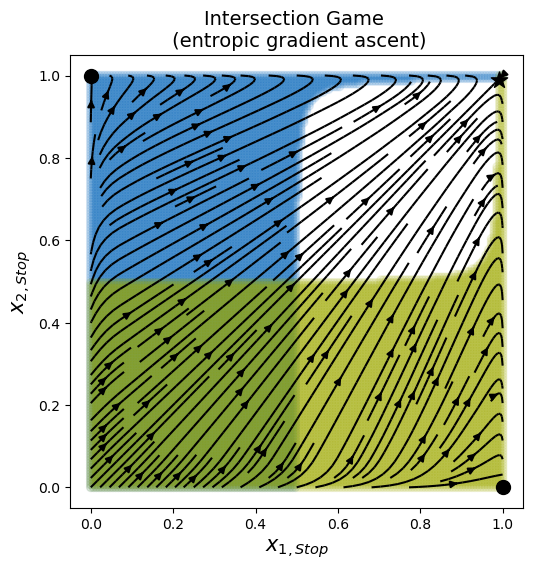
\includegraphics[width=\textwidth]{logos/Intersection4.png}
    \caption{stable neighbourhood w.r.t \textit{(Go,Stop)} in blue and w.r.t to \textit{(Stop,Go)} in light green}
    \label{fig:IntersectionGame1a}
\end{subfigure}%
\begin{subfigure}{.5\textwidth}
    \centering
    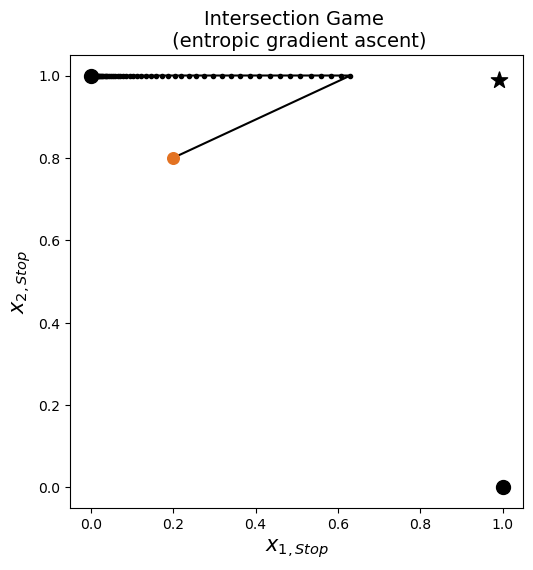
\includegraphics[width=\textwidth]{logos/Intersection5.png}
    \caption{$x_{1}^0 = (0.2,0.8)$, $x_{2}^0 = (0.8,0.2)$, \\ $T = 200$}
    \label{fig:IntersectionGame1b}
\end{subfigure}
\caption{EGA behavior in the Intersection game, $\gamma = 0.1$}
\label{fig:IntersectionGame1}
\end{figure}


Just like in Battle of Sexes we cannot find a neighborhood for the MNE such that the equation of the stability definition \ref{def:stability} is fulfilled. As we zoom in to the MNE again we cannot draw a circle around the MNE such that all points within the circle are colored. The zoomed in plot is analogue to \ref{fig:BOS3b} The same observations were made for POGA. 


\subsection{Coordination Game}\label{subsection:coordinationGame}

The behaviour of the Coordination game under no-regret dynamics has already been studied in \cite{jafari} but other no-regret algorithms than EGA and OPGA were used. As the name suggests, both player aim to cooperate, see table \ref{tab:payoffCoordination3x3}. 

\begin{table}[H]\centering
\setlength{\extrarowheight}{2pt}
\begin{tabular}{cc|c|c|c|}
  & \multicolumn{1}{c}{} & \multicolumn{1}{c}{$L$}  & \multicolumn{1}{c}{$C$}  & \multicolumn{1}{c}{$R$} \\\cline{3-5}
            & $T$ & $3,3$ & $0,0$ & $0,0$ \\ \cline{3-5}
            & $M$ & $0,0$ & $2,2$ & $0,0$ \\\cline{3-5}
            & $B$ & $0,0$ & $0,0$ & $1,1$ \\\cline{3-5}
\end{tabular}\caption{\label{tab:payoffCoordination3x3}payoff matrix Coordination Game}
\end{table}

There are three pure Nash equilibria and multiple fully mixed Nash equilibria. As we have seen in the previous examples fully mixed Nash equilibria are not stable therefore not learnable in general sum games under no-regret dynamics. For that reason we will neglect MNEs from now on. Lets consider the following three PNEs.

\begin{description}\centering
    \item $x^{*} = (T,L) \qquad \textit{strict }\text{PNE}$
    \item $x^{*} = (M,C) \qquad \textit{strict }\text{PNE}$
    \item $x^{*} = (B,R) \qquad \textit{strict }\text{PNE}$
\end{description}

Obviously all of them are strict PNEs as any unilateral deviation from an PNE results in a decrease in payoff. Note that \textit{(B,R)} is \textit{pareto dominated} by \textit{(M,C)} which is once again \textit{pareto dominated} by \textit{(T,L)}, so \textit{(T,L)} is \textit{pareto optimal}. \\

One might assume that for any general-sum game that is not zero-sum no-regret algorithms do not converge as we observed in the Shapley Game in subsection \ref{subsection:shapleyGame}. In the Coordination game however I found convergence to one of the above PNEs for all initial strategies. I have randomized the players' initail strategies and actually most of the time both algorithms converged to the \textit{pareto optimal} PNE \textit{(T,L)} (figure \ref{fig:Coordination3x3a}). Less often I found convergence to the PNE \textit{(M,C)} (figure \ref{fig:Coordination3x3b}) and even less often to the PNE \textit{(B,R)} (figure \ref{fig:Coordination3x3c}). Unfortunately I could not found a pattern for which initial strategy the algorithms converge to a specific PNE but the fact that most of the time it converges to \textit{(T,L)} might probably have something to do with its \textit{pareto dominance}. 

\begin{figure}[H]
\captionsetup{justification=centering}
\centering
\begin{subfigure}{.5\textwidth}
    \centering
    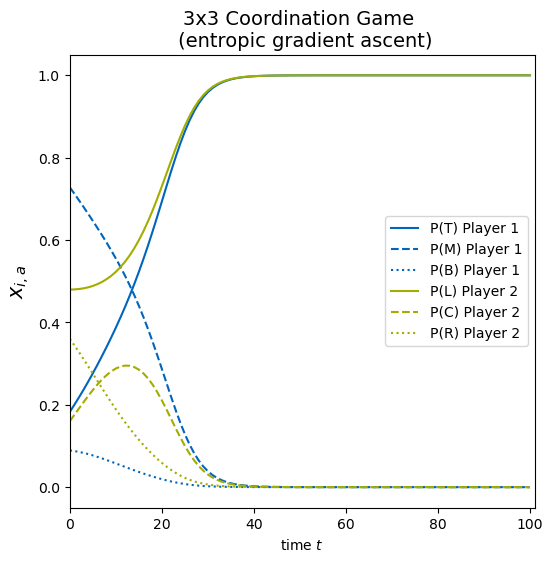
\includegraphics[width=\textwidth]{logos/Coordination3x3-1.png}
    \caption{convergence to \textit{(T,L)}}
    \label{fig:Coordination3x3a}
\end{subfigure}%
\begin{subfigure}{.5\textwidth}
    \centering
    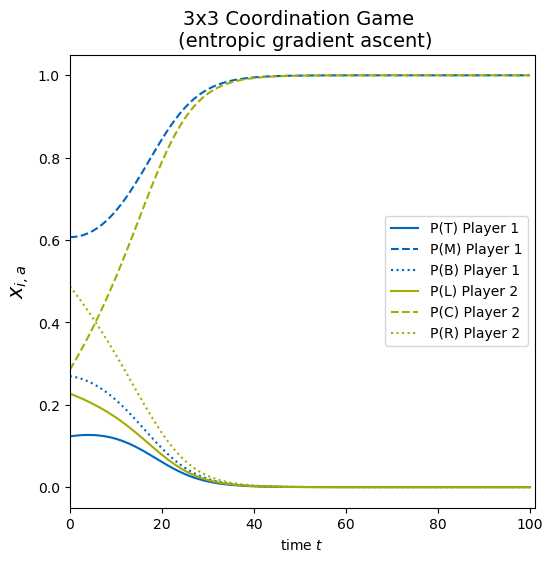
\includegraphics[width=\textwidth]{logos/Coordination3x3-2.png}
    \caption{convergence to \textit{(M,C)}}
    \label{fig:Coordination3x3b}
\end{subfigure}
\begin{subfigure}{.5\textwidth}
    \centering
    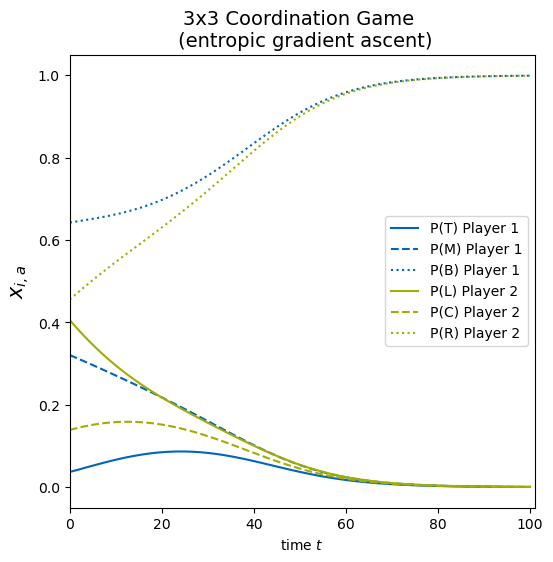
\includegraphics[width=\textwidth]{logos/Coordination3x3-3.png}
    \caption{convergence to \textit{(B,R)}}
    \label{fig:Coordination3x3c}
\end{subfigure}%
\caption{EGA behavior in the Coordination game, $\gamma = 0.1$}
\label{fig:Coordination3x3}
\end{figure}

The reason why both algorithms converge to Nash equilibria in the Coordination game and diverge in the Shapley Game is because there exists no strict NE in the Shapley Game but only an interior equilibrium. As we have concluded in chapter \ref{chapter:literatureReview} only strict NE survive under no-regret dynamics which means that in games where no strict NE exists we need to expect that the induced sequence of play diverges, as it did in the Shapley game. Note that empirical frequency of play might still converge even though no strict NE exists as we observed in the zero-sum games Matching Pennies and Rock Paper Scissors. 


\section{Strict and Weak Pure Nash Equilibria}\label{section:StrictandWeakPureNashEquilibria}

Lastly, I would like to address games that have a pure weak Nash equilibrium. As we have seen before the trajectories of both algorithms never converge to fully mixed Nash equilibria which are weak equilibria per definition. Nevertheless, games can be constructed such that they have pure strategy weak Nash equilibria. However they can only exist in the presence of another strict pure Nash equilibrium. When running the algorithms on such a game we find that as expected trajectories converge to the strict equilibrium locally. Interestingly though, I found divergent behavior for initial strategies that are \textit{close} to the weak equilibrium. 

\subsection{Two Player Two Strategies}\label{subsection:TwoPlayerTwoStrategies}

Consider the following 2x2 payoff matrix in table \ref{tab:payoffStrictAndWeak2x2}.

\begin{table}[H]\centering
\setlength{\extrarowheight}{2pt}
\begin{tabular}{cc|c|c|}
  & \multicolumn{1}{c}{} & \multicolumn{1}{c}{$H$}  & \multicolumn{1}{c}{$T$} \\\cline{3-4}
  & $H$ & $2,3$ & $1,2$ \\\cline{3-4}
  & $T$ & $1,2$ & $2,2$ \\\cline{3-4}
\end{tabular}\caption{\label{tab:payoffStrictAndWeak2x2}payoff matrix strict and weak Nash equilibria 2x2}
\end{table}

The game yields one fully mixed and two pure Nash equilibria. As the MNE is again not stable and as expected the sequence of play for both algorithms didn't converge to the MNE we will focus on the two PNEs. 

\begin{description}\centering
    \item $x^{*} = (H,H) \qquad \textit{strict }\text{PNE}$
    \item $x^{*} = (T,T) \qquad \textit{weak }\text{PNE}$
\end{description}

Lets first look at \textit{(H,H)}. It is strict in a sense of definition \ref{def:strictNE} as any unilateral deviation leads to a strict decrease in payoff. For instance, if the row player expects the column player to play \textit{H} then deviating from \textit{H} to \textit{T} would lead to a reduced payoff from $2$ to $1$. Similarly, expecting the row player to play \textit{H}, the column player's payoff decreases from $3$ to $2$ if the column player deviates from \textit{H} to \textit{T}. Therefore \textit{(H,H)} is a strict PNE. \\

\textit{(T,T)} on the other hand is weak. A PNE is called weak when there is no incentive for any player to unilaterally deviate but if they deviate then they do not necessarily reduce their payoff, or equivalently there exist more than one unique best response to the PNE. In the specific game above \textit{(T,T)} is weak because expecting the row player to play \textit{T} the row player can deviate from \textit{T} to \textit{H} without reducing its payoff as $2 \nless 2$. Note that \textit{(T,T)} is still an PNE as the payoff also doesn't strictly increase when deviating. \\

Now I would like to validate the results from chapter \ref{chapter:literatureReview} that only strict PNE survive under no-regret dynamics. For the strict PNE \textit{(H,H)} I found local stability as depicted by the blue region in figure \ref{fig:2x2Weak1}. As expected both algorithms converge to the strict PNE locally. However, even though it is the game's unique strict PNE, it is not globally stable as it was in the Prisoner's Dilemma. 

\begin{figure}[H]
\captionsetup{justification=centering}
\centering
\begin{subfigure}{.5\textwidth}
    \centering
    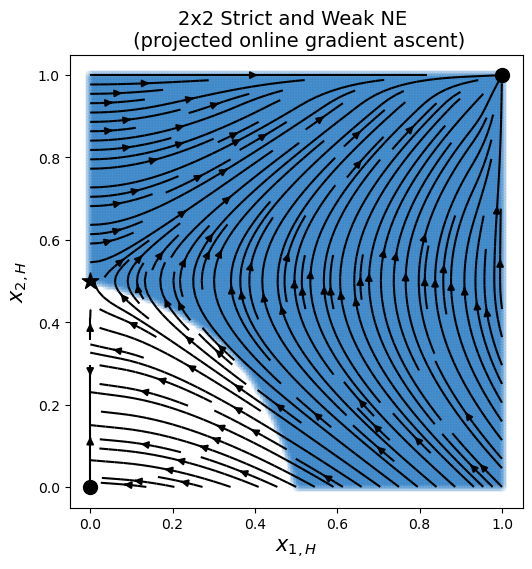
\includegraphics[width=\textwidth]{logos/Weak1.png}
    \caption{POGA}
    \label{fig:Weak1a}
\end{subfigure}%
\begin{subfigure}{.5\textwidth}
    \centering
    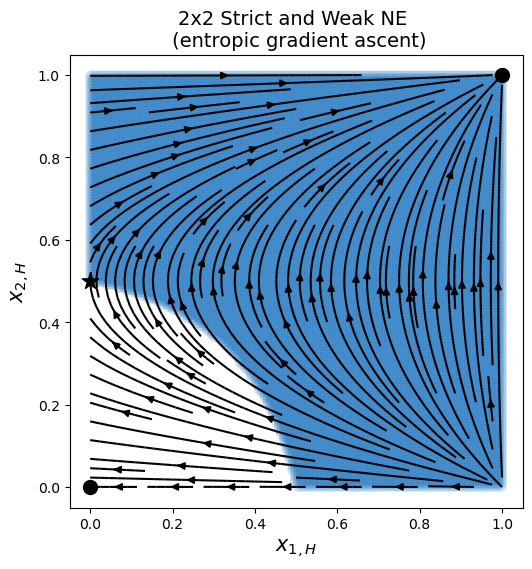
\includegraphics[width=\textwidth]{logos/Weak2.png}
    \caption{EGA}
    \label{fig:Weak1b}
\end{subfigure}
\caption{vector field with stable neighbourhood w.r.t strict PNE \textit{(H,H)} colored in blue}
\label{fig:2x2Weak1}
\end{figure}

A closer look at the weak PNE \textit{(T,T)} shows that it is not stable in a sense of definition \ref{def:stability}. There are always strategies in the neighborhood of the weak PNE that did not fulfill the inequality of the definition. Especially strategies profile where the row player played \textit{T} with probability $1$ and \textit{H} with probability $0$ I found gaps that were not stable with respect to the weak PNE no matter how much we zoom in, see figure \ref{fig:Weak2b}. Blue points indicate strategy profiles for which the inequality from the stability definition holds. This observations fits proposition \ref{prop:StrictStableEquivalent} saying that only strict PNEs are stable. The same results were found for POGA. \\

\begin{figure}[H]
\captionsetup{justification=centering}
\centering
\begin{subfigure}{.48\textwidth}
    \centering
    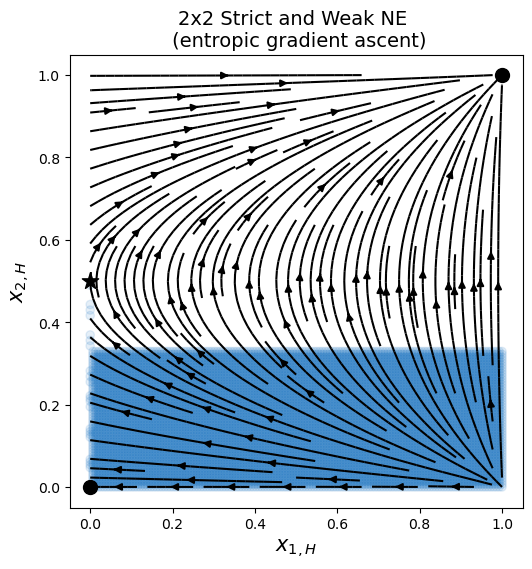
\includegraphics[width=\textwidth]{logos/Weak3.png}
    \caption{stable neighbourhood w.r.t \textit{(T,T)}}
    \label{fig:Weak2a}
\end{subfigure}%
\begin{subfigure}{.52\textwidth}
    \centering
    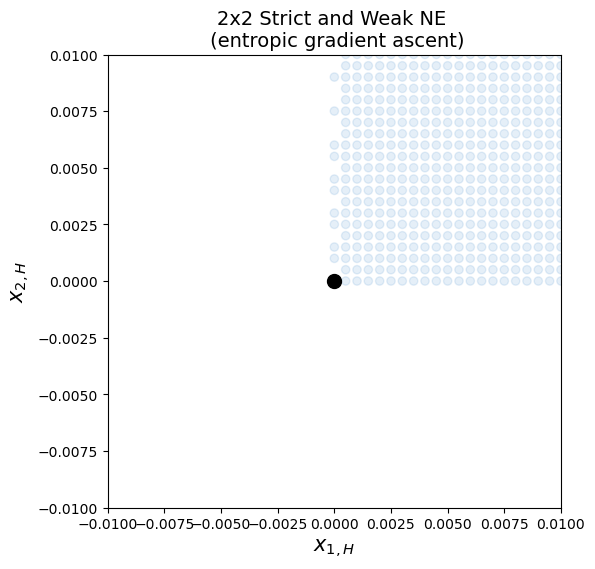
\includegraphics[width=\textwidth]{logos/Weak4.png}
    \caption{zoomed in to \textit{(T,T)}}
    \label{fig:Weak2b}
\end{subfigure}
\caption{The weak PNE \textit{(T,T)} is not stable under EGA}
\label{fig:2x2Weak2}
\end{figure}

The vector fields might be misleading though as it looks like the EGA algorithm steps outside the feasible probability simplex. A closer examination however showed that for some initial strategies that are locally close to the weak PNE, the EGA algorithm diverges towards the "left wall". An example trajectory for that phenomena is shown in figure \ref{fig:Weak3a}. No matter how much iterations were used, the EGA algorithm didn't change its direction. Changing the initial strategy slightly closer towards the strict PNE, however, yields convergence as illustrated in \ref{fig:Weak3b}. Again, the some holds for POGA.

\begin{figure}[H]
\captionsetup{justification=centering}
\centering
\begin{subfigure}{.5\textwidth}
    \centering
    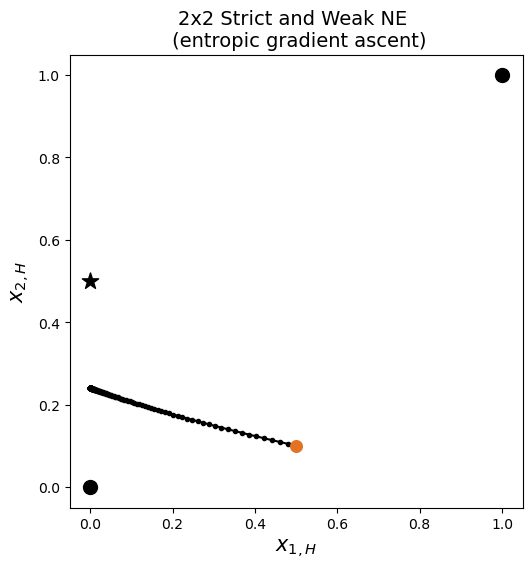
\includegraphics[width=\textwidth]{logos/Weak5.png}
    \caption{$x_{1}^0 = (0.5,0.5)$, $x_{2}^0 = (0.1,0.9)$, $T = 200$}
    \label{fig:Weak3a}
\end{subfigure}%
\begin{subfigure}{.5\textwidth}
    \centering
    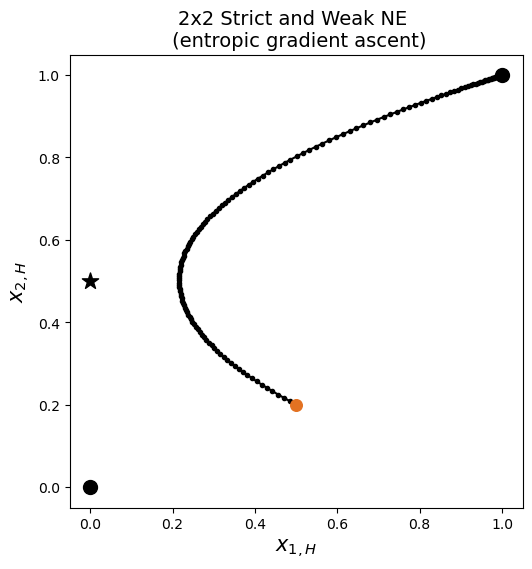
\includegraphics[width=\textwidth]{logos/Weak6.png}
    \caption{$x_{1}^0 = (0.5,0.5)$, $x_{2}^0 = (0.2,0.8)$, $T = 200$}
    \label{fig:Weak3b}
\end{subfigure}
\caption{divergent and convergent behavior using EGA, $\gamma = 0.1$}
\label{fig:2x2Weak3}
\end{figure}

So indeed the strict and therefore stable PNE is also locally attracting (proposition \ref{prop:localConvergence}). But even though there exists a unique strict PNE, as in the Prisoner's Dilemma, this game shows that no-regret dynamics do not converge to it globally. It seems like the existence of a weak PNE is disrupting the convergence to the strict PNE. Also its worth mentioning that for no initial strategy I have found convergence to the weak PNE but rather divergence towards the "left wall". I came to the same conclusions for both algorithms.


\subsection{Two Player Three Strategies}\label{subsection:TwoPlayerThreeStrategies}

The following game is a 3x3 general-sum game that has two strict and one weak pure Nash equilibria. There are also multiple fully mixed Nash equilibria but they are neglected again as the sequence of play never converges to one of them for the very same reason that interior states cannot be stable and therefore not attracting under no-regret dynamics (proposition \ref{prop:noInteriorStable}). Consider the 3x3 payoff matrix described in table \ref{tab:payoffStrictAndWeak3x3}. 

\begin{table}[H]\centering
\setlength{\extrarowheight}{2pt}
\begin{tabular}{cc|c|c|c|}
  & \multicolumn{1}{c}{} & \multicolumn{1}{c}{$A$}  & \multicolumn{1}{c}{$B$}  & \multicolumn{1}{c}{$C$} \\\cline{3-5}
            & $X$ & $2,3$ & $1,2$ & $1,1$ \\ \cline{3-5}
            & $Y$ & $1,1$ & $2,1$ & $3,2$ \\\cline{3-5}
            & $Z$ & $1,2$ & $2,2$ & $2,1$ \\\cline{3-5}
\end{tabular}\caption{\label{tab:payoffStrictAndWeak3x3}payoff matrix strict and weak Nash equilibria 3x3}
\end{table}

The three pure Nash equilibria are

\begin{description}\centering
    \item $x^{*} = (X,A) \qquad \textit{strict }\text{PNE}$
    \item $x^{*} = (Y,C) \qquad \textit{strict }\text{PNE}$
    \item $x^{*} = (Z,B) \qquad \textit{weak }\text{PNE}$
\end{description}

One can easily check that \textit{(X,A)} and \textit{(Y,B)} are strict as they are unique best responses. \textit{(Z,B)} however is not a unique best response for the column player. Assuming the row player to choose \textit{Z}, the column player can deviate from \textit{B} to \textit{A} without loosing any payoff. The payoff for the column player stays at $2$ for that deviation. Therefore \textit{(Z,B)} is weak. \\

As far as convergence is concerned I found similar result as in the 2x2 game discussed previously. The initial strategies were randomized. In every case I found convergence of both EGA and OPGA to one of the strict PNE. Figure \ref{fig:Weak3x3a} shows an example for convergence to \textit{(X,A)}. Less often I found convergence to the other strict PNE \textit{(Y,B)}, see an example in figure \ref{fig:Weak3x3b}. 

\begin{figure}[H]
\captionsetup{justification=centering}
\centering
\begin{subfigure}{.5\textwidth}
    \centering
    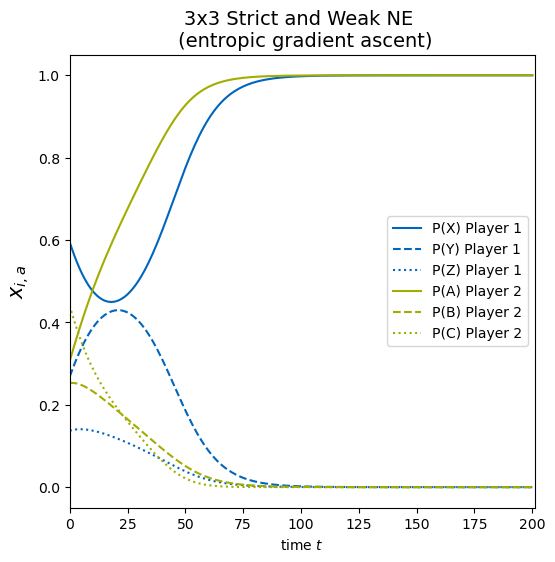
\includegraphics[width=\textwidth]{logos/Weak3x3a.png}
    \caption{convergence to \textit{(X,A)}}
    \label{fig:Weak3x3a}
\end{subfigure}%
\begin{subfigure}{.5\textwidth}
    \centering
    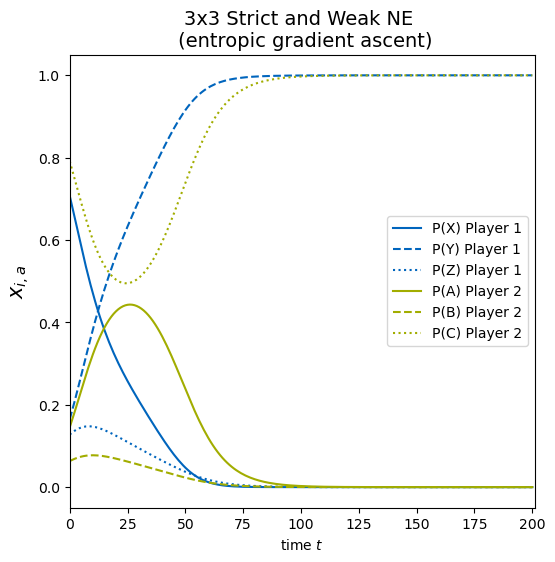
\includegraphics[width=\textwidth]{logos/Weak3x3b.png}
    \caption{convergence to \textit{(Y,B)}}
    \label{fig:Weak3x3b}
\end{subfigure}
\caption{Convergent behavior for strict PNE using EGA, $\gamma = 0.1$}
\label{fig:Weak3x3}
\end{figure}

For non of the tested initial strategy profiles I found convergence to neither the weak PNE \textit{(Z,B)} nor any of the fully mixed NE. Again these empirical findings match the general result that under no-regret dynamics only strict Nash equilibria survive.  
